\documentclass[t,aspectratio=169,xcolor=dvipsnames]{beamer}

\usepackage{hyperref}
\usepackage{graphicx}
\usepackage{booktabs}
\usepackage{tikz}
\usetikzlibrary{shapes,arrows,positioning,calc,matrix}
\usepackage{makecell}
\newcommand*{\defeq}{\stackrel{\text{def}}{=}}
\usepackage{setspace}
\usepackage[utf8]{inputenc}
\usepackage[T1]{fontenc}
\usepackage{helvet}
\usepackage{amsmath,amssymb,amsfonts}
\usepackage{bm}
\usepackage{ragged2e}
\usepackage{xfrac}
\usepackage[loose]{units}
\usepackage{braket}
\usepackage{gensymb}
\usepackage{verbatim}
\usepackage{fancyvrb}
\usepackage{listings}
\usepackage{xcolor}

% --- Minimalist Color Palette (DESIGN.md) ---
\definecolor{dlInk}{HTML}{111111}
\definecolor{dlCanvas}{HTML}{FFFFFF}
\definecolor{dlSoftCloud}{HTML}{F5F5F5}
\definecolor{dlCharcoal}{HTML}{39393B}
\definecolor{dlMute}{HTML}{707072}
\definecolor{dlHairline}{HTML}{CACACB}
\definecolor{dlTeal}{HTML}{0A7281}
\definecolor{nyublue}{HTML}{0A7281}
\definecolor{codeBg}{HTML}{F7F7F8}

% --- Beamer Theme Customization ---
\usetheme{default}
\useinnertheme{rectangles}
\setbeamertemplate{navigation symbols}{}

\setbeamercolor{palette primary}{bg=dlInk,fg=dlCanvas}
\setbeamercolor{palette secondary}{bg=dlCharcoal,fg=dlCanvas}
\setbeamercolor{palette tertiary}{bg=dlSoftCloud,fg=dlInk}
\setbeamercolor{structure}{fg=dlInk}
\setbeamercolor{title}{fg=dlCanvas,bg=dlInk}
\setbeamercolor{frametitle}{fg=dlInk,bg=dlSoftCloud}
\setbeamercolor{normal text}{fg=dlInk,bg=dlCanvas}
\setbeamercolor{block title}{bg=dlInk,fg=dlCanvas}
\setbeamercolor{block body}{bg=dlSoftCloud,fg=dlInk}
\setbeamercolor{block title example}{bg=dlTeal,fg=dlCanvas}
\setbeamercolor{block body example}{bg=dlSoftCloud,fg=dlInk}
\setbeamercolor{block title alert}{bg=dlCharcoal,fg=dlCanvas}
\setbeamercolor{block body alert}{bg=dlSoftCloud,fg=dlInk}
\setbeamercolor{item}{fg=dlInk}

\makeatletter
\setbeamertemplate{frametitle}{%
  \nointerlineskip%
  \begin{beamercolorbox}[wd=\paperwidth,ht=3.8ex,dp=1.5ex,leftskip=1.0cm,rightskip=1.0cm]{frametitle}%
    \textbf{\large\strut\insertframetitle}%
    \ifx\insertframesubtitle\@empty\else\hfill{\footnotesize\color{dlMute}\insertframesubtitle}\fi%
  \end{beamercolorbox}%
}
\makeatother

\setbeamertemplate{footline}{%
  \begin{beamercolorbox}[wd=\paperwidth,ht=2.5ex,dp=1.2ex,leftskip=1.0cm,rightskip=1.0cm]{palette primary}%
    \tiny\textbf{IF25-40401 · Deep Learning} \hfill \insertshorttitle \hfill \textbf{\insertframenumber{} / \inserttotalframenumber}%
  \end{beamercolorbox}%
}

\lstset{
  backgroundcolor=\color{codeBg},
  basicstyle=\ttfamily\scriptsize\color{dlInk},
  keywordstyle=\bfseries\color{dlTeal},
  commentstyle=\color{dlMute}\itshape,
  stringstyle=\color{dlCharcoal},
  breaklines=true,
  frame=single,
  rulecolor=\color{dlHairline},
  numbers=none,
  tabsize=2,
  showstringspaces=false
}

\title[Pertemuan 4: CNN From Scratch]{Deep Learning (IF25-40401)} 
\subtitle{Pertemuan 4: CNN From Scratch}
\author{Tim Dosen Deep Learning}
\institute{Teknik Informatika — Institut Teknologi Sumatera (ITERA)}
\date{2026}

\begin{document}

% --- TITLE SLIDE (Minimalist Campaign Style) ---
\begin{frame}[plain]
  \begin{beamercolorbox}[wd=\paperwidth,ht=\paperheight,sep=1.5cm]{palette primary}
    \vspace{0.8cm}
    {\scriptsize\bfseries\color{dlMute}IF25-40401 · DEEP LEARNING · PERTEMUAN 04}\\[0.4cm]
    {\Huge\bfseries DEEP COMPUTER VISION (1):\\CNN FROM SCRATCH}\\[0.4cm]
    {\small Konvolusi, Stride, Padding, Pooling, Receptive Field, dan Implementasi PyTorch LeNet}\\[1.0cm]
    \vfill
    {\scriptsize\textbf{Tim Dosen Deep Learning} · Institut Teknologi Sumatera (ITERA)}
  \end{beamercolorbox}
\end{frame}

%------------------------------------------------
%	LEARNING OBJECTIVES SLIDE
%------------------------------------------------
\begin{frame}[plain]

    \frametitle{TUJUAN PEMBELAJARAN} 
    \framesubtitle{Capaian Pembelajaran Pertemuan 4 (RPS IF25-40401)}

    \begin{exampleblock}{Setelah mengikuti pertemuan ini, mahasiswa diharapkan mampu:}
        \begin{enumerate}
            \item \textbf{Menjelaskan operasi konvolusi, stride, padding, dan pooling} dalam ekstraksi representasi spasial citra
            \item \textbf{Menghitung ukuran feature map dan jumlah parameter konvolusi} secara terstruktur
            \item \textbf{Membangun dan melatih CNN dari nol} menggunakan framework PyTorch
            \item \textbf{Menganalisis peran weight sharing dan konektivitas lokal} dalam mengatasi keterbatasan MLP
        \end{enumerate}
    \end{exampleblock}
    
\end{frame}

%------------------------------------------------
%	OUTLINE SLIDE
%------------------------------------------------
\begin{frame}[plain]

    \frametitle{OUTLINE} 
    \framesubtitle{~}

    \begin{spacing}{1.2}
        \tableofcontents
    \end{spacing}
    
\end{frame}

\section{Review: Neural Network}

\begin{frame}[plain]
  \begin{beamercolorbox}[wd=\paperwidth,ht=\paperheight,sep=1.5cm]{palette primary}
    \vspace{1.5cm}
    {\scriptsize\bfseries\color{dlMute}BAGIAN 01 · REVIEW}\\[0.4cm]
    {\Huge\bfseries Review: Neural Network}\\[0.4cm]
    {\small\color{dlHairline}Fondasi Deep Learning}
    \vfill
  \end{beamercolorbox}
\end{frame}

%------------------------------------------------
%	NEW SLIDE
%------------------------------------------------
\begin{frame}
    \frametitle{Neural Network}
    \framesubtitle{Fondasi Pembelajaran Mesin}
    \small
    \begin{block}{Apa itu Neural Network?}
        \textbf{Neural Network} adalah model komputasi yang terinspirasi dari cara kerja otak manusia, terdiri dari \textbf{neuron buatan} yang saling terhubung untuk memproses informasi dan belajar dari data.
    \end{block}

    \begin{columns}[t]
        \column{0.48\textwidth}
        \textbf{Komponen Utama:}
        \begin{itemize}
            \item \textbf{Input Layer:} Menerima data
            \item \textbf{Hidden Layer:} Memproses informasi
            \item \textbf{Output Layer:} Menghasilkan prediksi
            \item \textbf{Weights \& Biases:} Parameter pembelajaran
        \end{itemize}

        \column{0.48\textwidth}
        \textbf{Fungsi Utama:}
        \begin{itemize}
            \item \textbf{Pattern Recognition:} Mengenali pola dalam data
            \item \textbf{Classification:} Mengklasifikasi data
            \item \textbf{Regression:} Memprediksi nilai kontinu
            \item \textbf{Feature Learning:} Belajar fitur otomatis
        \end{itemize}
    \end{columns}

\end{frame}

%------------------------------------------------
%	NEW SLIDE
%------------------------------------------------
\begin{frame}
    \frametitle{Interactive Backpropagation Visualization}
    \framesubtitle{Understanding Neural Network Learning Process}

    \begin{exampleblock}{Explore Neural Networks Interactively}
        Untuk memahami lebih dalam bagaimana \textbf{backpropagation} bekerja dalam neural network, kita dapat menggunakan visualisasi interaktif yang memungkinkan eksplorasi real-time dari proses pembelajaran.
    \end{exampleblock}

    \begin{center}
        \large
        \textbf{Interactive Demo:}\\[0.5cm]
        \textcolor{blue}{\url{https://xnought.github.io/backprop-explainer/}}
    \end{center}

    \textbf{Fitur Visualisasi:}
    \begin{itemize}
        \item \textbf{Real-time computation:} Lihat bagaimana gradient dihitung
        \item \textbf{Interactive parameters:} Ubah weights dan bias secara langsung
        \item \textbf{Visual backpropagation:} Animasi aliran gradient melalui network
        \item \textbf{Step-by-step learning:} Pahami setiap tahap forward dan backward pass
    \end{itemize}

\end{frame}

%------------------------------------------------
%	NEW SLIDE
%------------------------------------------------
\begin{frame}
    \frametitle{Proses Pembelajaran Neural Network}
    \framesubtitle{Forward Propagation dan Backpropagation}

    \begin{exampleblock}{Tahapan Pembelajaran}
        Neural Network belajar melalui proses \textbf{iteratif} yang melibatkan \textbf{forward propagation} untuk menghasilkan prediksi dan \textbf{backpropagation} untuk memperbarui parameter berdasarkan kesalahan.
    \end{exampleblock}

    \begin{columns}[t]
        \column{0.48\textwidth}
        \textbf{Forward Propagation:}
        \begin{itemize}
            \item Data input diproses layer demi layer
            \item Setiap neuron menerapkan \textbf{fungsi aktivasi}
            \item Menghasilkan \textbf{output/prediksi} akhir
            \item Menghitung \textbf{loss function}
        \end{itemize}

        \column{0.48\textwidth}
        \textbf{Backpropagation:}
        \begin{itemize}
            \item Menghitung \textbf{gradient} dari loss function
            \item Memperbarui \textbf{weights} dan \textbf{biases}
            \item Menggunakan \textbf{chain rule} untuk propagasi error
            \item Optimasi dengan \textbf{gradient descent}
        \end{itemize}
    \end{columns}

\end{frame}

%------------------------------------------------
%	NEW SLIDE
%------------------------------------------------
\begin{frame}
    \frametitle{Tantangan Neural Network Tradisional}
    \framesubtitle{Keterbatasan untuk Data Visual}
    \small

    \begin{alertblock}{Masalah Utama}
        Neural Network tradisional (\textbf{Fully Connected}) memiliki keterbatasan signifikan dalam memproses \textbf{data visual} seperti gambar karena tidak mempertimbangkan \textbf{struktur spasial} dan \textbf{lokalitas} informasi.
    \end{alertblock}

    \begin{columns}[t]
        \column{0.48\textwidth}
        \textbf{Keterbatasan Teknis:}
        \begin{itemize}
            \item \textbf{Dimensi tinggi:} Gambar 28x28 = 784 parameter
            \item \textbf{Overfitting:} Terlalu banyak parameter
            \item \textbf{Translation invariance:} Tidak robust terhadap pergeseran
            \item \textbf{Komputasi mahal:} Banyak koneksi tidak perlu
        \end{itemize}

        \column{0.48\textwidth}
        \textbf{Masalah Struktural:}
        \begin{itemize}
            \item Tidak memahami \textbf{hierarki fitur}
            \item Kehilangan informasi \textbf{spasial}
            \item Tidak efisien untuk \textbf{pattern lokal}
            \item Sulit mendeteksi \textbf{fitur visual} kompleks
        \end{itemize}
    \end{columns}

\end{frame}

%------------------------------------------------
%	NEW SLIDE
%------------------------------------------------
\begin{frame}
    \frametitle{Solusi: Convolutional Neural Network (CNN)}
    \framesubtitle{Arsitektur yang Dirancang untuk Data Visual}
    \small
    \begin{exampleblock}{Inovasi CNN}
        \textbf{Convolutional Neural Network (CNN)} adalah evolusi dari neural network tradisional yang dirancang khusus untuk memproses data visual dengan memanfaatkan \textbf{operasi konvolusi} dan \textbf{struktur spasial} gambar.
    \end{exampleblock}
    \footnotesize

    \begin{columns}[t]
        \column{0.48\textwidth}
        \textbf{Keunggulan CNN:}
        \begin{itemize}
            \item \textbf{Local connectivity:} Koneksi lokal, bukan global
            \item \textbf{Parameter sharing:} Filter yang sama untuk seluruh gambar
            \item \textbf{Translation invariance:} Robust terhadap pergeseran
            \item \textbf{Hierarki fitur:} Dari sederhana ke kompleks
        \end{itemize}

        \column{0.48\textwidth}
        \textbf{Komponen Utama CNN:}
        \begin{itemize}
            \item \textbf{Convolutional Layer:} Ekstraksi fitur lokal
            \item \textbf{Pooling Layer:} Reduksi dimensi
            \item \textbf{Activation Function:} Non-linearitas
            \item \textbf{Fully Connected Layer:} Klasifikasi akhir
        \end{itemize}
    \end{columns}

\end{frame}

%------------------------------------------------
%	NEW SLIDE
%------------------------------------------------
\begin{frame}
    \frametitle{Mengapa CNN Revolusioner?}
    \framesubtitle{Dampak pada Computer Vision dan AI}
    \small

    \begin{block}{Revolusi dalam Pemrosesan Visual}
        CNN telah mengubah lanskap \textbf{computer vision} dan \textbf{artificial intelligence}, memungkinkan terobosan dalam \textbf{image recognition}, \textbf{object detection}, dan berbagai aplikasi visual lainnya yang sebelumnya tidak mungkin dilakukan.
    \end{block}

    \begin{columns}[t]
        \column{0.48\textwidth}
        \textbf{Aplikasi Real-world:}
        \begin{itemize}
            \item \textbf{Medical imaging:} Diagnosis kanker, X-ray
            \item \textbf{Autonomous vehicles:} Deteksi objek
            \item \textbf{Face recognition:} Keamanan dan autentikasi
            \item \textbf{Social media:} Auto-tagging, filter
        \end{itemize}

        \column{0.48\textwidth}
        \textbf{Milestone Penting:}
        \begin{itemize}
            \item \textbf{ImageNet 2012:} AlexNet mengalahkan metode tradisional
            \item \textbf{Akurasi tinggi:} > 95\% pada image classification
            \item \textbf{Transfer learning:} Model pre-trained
            \item \textbf{Deep learning boom:} Memicu era AI modern
        \end{itemize}
    \end{columns}
\end{frame}

%------------------------------------------------
%	NEW SLIDE: MLP LIMITATIONS & PARAMETER EXPLOSION
%------------------------------------------------
\begin{frame}
    \frametitle{Keterbatasan MLP: Analisis Ledakan Parameter}
    \framesubtitle{Mengapa Fully Connected Layer Gagal pada Citra?}
    \footnotesize

    \begin{alertblock}{Masalah Utama Multilayer Perceptron (MLP) pada Citra}
        \textbf{Kehilangan Struktur Spasial:} Citra di-\textit{flatten} 1D, merusak relasi piksel tetangga. \\
        \textbf{Ledakan Parameter:} Setiap neuron terhubung ke seluruh piksel input.
    \end{alertblock}

    \begin{columns}[t]
        \column{0.48\textwidth}
        \textbf{Perhitungan Parameter MLP:}
        \begin{itemize}
            \item Citra CIFAR-10 ($32\times32\times3 = 3.072$):
            $$\text{Bobot} = 3.072 \times 1.024 \approx \mathbf{3{,}14\text{ juta}}$$
            \item Resolusi $224\times224\times3 = 150.528$:
            $$\text{Bobot} = 150.528 \times 1.024 \approx \mathbf{154\text{ juta}}$$
            \item \textit{Hanya untuk layer pertama saja!}
        \end{itemize}

        \column{0.48\textwidth}
        \textbf{Dampak Negatif:}
        \begin{itemize}
            \item \textbf{Severe Overfitting:} Kapasitas model berlebihan untuk dataset kecil.
            \item \textbf{Sensitivitas Translasi:} Geser 1 piksel mengubah vektor input sepenuhnya.
            \item \textbf{Beban Komputasi:} Sangat boros memori GPU/RAM.
        \end{itemize}
    \end{columns}
\end{frame}

%------------------------------------------------
%	NEW SLIDE: LOCAL CONNECTIVITY & WEIGHT SHARING
%------------------------------------------------
\begin{frame}
    \frametitle{Dua Pilar Solusi CNN: Local Connectivity \& Weight Sharing}
    \framesubtitle{Fondasi Efisiensi Representasi Spasial (CS231n)}
    \footnotesize

    \begin{columns}[t]
        \column{0.48\textwidth}
        \begin{block}{1. Local Connectivity}
            \textbf{Konektivitas Lokal:}
            \begin{itemize}
                \item Tiap neuron hanya terhubung ke sub-wilayah kecil (\textbf{local receptive field}), misal $3\times3$ atau $5\times5$.
                \item \textit{Rasional:} Piksel bertetangga memiliki korelasi tinggi (tepi, tekstur, kontur).
                \item Menjaga topologi spasial 2D citra.
            \end{itemize}
        \end{block}

        \column{0.48\textwidth}
        \begin{exampleblock}{2. Weight Sharing}
            \textbf{Pembagian Bobot:}
            \begin{itemize}
                \item Kumpulan bobot filter yang sama digeser (\textit{slide}) ke seluruh citra.
                \item \textit{Rasional (Stationarity):} Fitur berguna di sudut kiri juga berguna di sudut kanan.
                \item \textbf{Efek:} Filter $5\times5\times3$ (16 filter) hanya butuh \textbf{1.216 bobot} (hemat $>99.9\%$).
            \end{itemize}
        \end{exampleblock}
    \end{columns}

\end{frame}

\section{History of CNN}

%------------------------------------------------
%	SECTION TITLE SLIDE
%------------------------------------------------
\begin{frame}[plain]
  \begin{beamercolorbox}[wd=\paperwidth,ht=\paperheight,sep=1.5cm]{palette primary}
    \vspace{1.5cm}
    {\scriptsize\bfseries\color{dlMute}BAGIAN 02 · HISTORI}\\[0.4cm]
    {\Huge\bfseries History of CNN}\\[0.4cm]
    {\small\color{dlHairline}Evolusi Convolutional Neural Network dari 1960s hingga Era Modern}
    \vfill
  \end{beamercolorbox}
\end{frame}

%------------------------------------------------
%	NEW SLIDE
%------------------------------------------------
\begin{frame}
    \frametitle{Era Fondasi: Dari Biologi ke Model Kerja}
    \framesubtitle{1960s - 1998}
    \small

    \begin{block}{Inspirasi Biologis (1960s)}
        \textbf{Hubel \& Wiesel} menemukan struktur hierarkis visual cortex kucing yang menjadi blueprint CNN - neuron sederhana mendeteksi tepi, neuron kompleks mendeteksi bentuk yang lebih rumit.
    \end{block}

    \begin{columns}[t]
        \column{0.48\textwidth}
        \textbf{1980 - Neocognitron (Fukushima):}
        \begin{itemize}
            \item Leluhur pertama CNN modern
            \item Memperkenalkan \textbf{convolutional layers} (S-cells)
            \item Menggunakan \textbf{pooling layers} (C-cells)
            \item Keterbatasan: belum ada backpropagation
        \end{itemize}

        \column{0.48\textwidth}
        \textbf{1989-1998 - LeNet-5 (Yann LeCun):}
        \begin{itemize}
            \item CNN praktis pertama dengan \textbf{backpropagation}
            \item Digunakan untuk \textbf{pembacaan cek otomatis}
            \item Struktur: Conv - Pool - Conv - Pool - FC
            \item Sukses komersial pertama CNN
        \end{itemize}
    \end{columns}
\end{frame}

%------------------------------------------------
%	NEW SLIDE
%------------------------------------------------
\begin{frame}
    \frametitle{AI Winter dan Masa Inkubasi}
    \framesubtitle{Late 1990s - 2011}
    \small

    \begin{alertblock}{Periode Sunyi CNN}
        Selama lebih dari satu dekade, CNN kehilangan popularitas mainstream. Kebutuhan komputasi yang besar dan dominasi metode lain seperti \textbf{Support Vector Machines (SVMs)} membuat CNN tertinggal.
    \end{alertblock}
    \footnotesize

    \begin{columns}[t]
        \column{0.48\textwidth}
        \textbf{Tantangan Era Ini:}
        \begin{itemize}
            \item \textbf{Keterbatasan komputasi:} CPU tidak cukup kuat
            \item \textbf{Dataset kecil:} Belum ada ImageNet
            \item \textbf{Kompetisi ketat:} SVM lebih efektif
            \item \textbf{Training lambat:} Optimasi belum matang
        \end{itemize}

        \column{0.48\textwidth}
        \textbf{Persiapan Revolusi:}
        \begin{itemize}
            \item \textbf{Riset berlanjut:} Perbaikan arsitektur
            \item \textbf{Pengembangan GPU:} NVIDIA CUDA
            \item \textbf{Dataset besar:} Persiapan ImageNet
            \item \textbf{Algoritma baru:} Inovasi training
        \end{itemize}
    \end{columns}

    \begin{exampleblock}{Menanti Momentum}
        Periode ini mempersiapkan dua ingredien kunci untuk revolusi CNN: \textbf{massive datasets} dan \textbf{powerful GPUs}.
    \end{exampleblock}
\end{frame}

%------------------------------------------------
%	NEW SLIDE
%------------------------------------------------
\begin{frame}
    \frametitle{Era Keemasan: Revolusi Deep Learning}
    \framesubtitle{2012 - 2020}
    \footnotesize

    \begin{exampleblock}{2012 - Big Bang: AlexNet}
        AlexNet menghancurkan kompetisi ImageNet dengan error rate \textbf{15.3\%} vs \textbf{26.2\%} (runner-up), memicu revolusi deep learning dan menempatkan CNN di garis depan AI.
    \end{exampleblock}

    \begin{columns}[t]
        \column{0.48\textwidth}
        \textbf{Inovasi AlexNet:}
        \begin{itemize}
            \item \textbf{ReLU activation:} Training lebih cepat
            \item \textbf{Dropout:} Mencegah overfitting
            \item \textbf{GPU training:} Memanfaatkan parallelisasi
            \item \textbf{Deep architecture:} 8 layers
        \end{itemize}

        \column{0.48\textwidth}
        \textbf{2014-2015 - Arms Race:}
        \begin{itemize}
            \item \textbf{VGGNet:} Deeper dengan 3x3 conv uniform
            \item \textbf{GoogLeNet:} Inception modules paralel
            \item \textbf{ResNet (2015):} Skip connections, 152+ layers
            \item \textbf{Vanishing gradient:} Diselesaikan ResNet
        \end{itemize}
    \end{columns}
    \vspace{0.3cm}
    \textbf{2016-2020:} Refinement era dengan DenseNet, MobileNet (efficiency), EfficientNet (systematic scaling).
\end{frame}

%------------------------------------------------
%	NEW SLIDE
%------------------------------------------------
\begin{frame}
    \frametitle{Tantangan Baru: Era Transformer}
    \framesubtitle{2020 - 2022}
    \footnotesize

    \begin{alertblock}{Kedatangan Kompetitor Kuat}
        \textbf{Vision Transformer (ViT)} mengadaptasi arsitektur Transformer dari NLP ke computer vision, mengancam dominasi CNN dengan performa superior pada dataset besar.
    \end{alertblock}

    \begin{columns}[t]
        \column{0.48\textwidth}
        \textbf{2020 - Vision Transformer (ViT):}
        \begin{itemize}
            \item Memecah image menjadi \textbf{patches}
            \item Menggunakan \textbf{self-attention mechanism}
            \item Unggul pada dataset besar (JFT-300M)
            \item Melampaui performa top CNNs
        \end{itemize}

        \column{0.48\textwidth}
        \textbf{2021-2022 - Dominasi Transformer:}
        \begin{itemize}
            \item \textbf{Swin Transformer:} Lebih efisien
            \item \textbf{State-of-the-art:} Berbagai benchmark vision
            \item \textbf{Narratif baru:} "Attention is all you need"
            \item \textbf{CNN terancam:} Prediksi akan tergantikan
        \end{itemize}
    \end{columns}

    \begin{block}{Momentum Transformer}
        Komunitas AI mulai mempertanyakan relevansi CNN dengan fixed, local inductive bias vs global attention Transformer.
    \end{block}
\end{frame}

%------------------------------------------------
%	NEW SLIDE
%------------------------------------------------
\begin{frame}
    \frametitle{Trivia: Transformer Revolution}
    \framesubtitle{Paper yang Mengubah Dunia AI}
    \scriptsize

    \begin{exampleblock}{2017 - "Attention Is All You Need"}
        Paper revolusioner dari Google Brain yang memperkenalkan \textbf{Transformer architecture} - awalnya untuk machine translation, namun tanpa disadari telah meletakkan fondasi untuk \textbf{era AI generatif} modern.
    \end{exampleblock}

    \begin{columns}[t]
        \column{0.48\textwidth}
        \textbf{Kelahiran GPT Lineage:}
        \begin{itemize}
            \item \textbf{2018 - GPT-1:} OpenAI adopsi Transformer
            \item \textbf{2019 - GPT-2:} "Too dangerous to release"
            \item \textbf{2020 - GPT-3:} 175B parameters, emergence
            \item \textbf{2022 - ChatGPT:} Mengubah persepsi publik AI
        \end{itemize}

        \column{0.48\textwidth}
        \textbf{Dominasi Cross-Modal:}
        \begin{itemize}
            \item \textbf{NLP:} BERT, T5, GPT series
            \item \textbf{Vision:} ViT, DALL-E, Stable Diffusion
            \item \textbf{Multimodal:} GPT-4V, Gemini
            \item \textbf{Foundation models:} Paradigma baru AI
        \end{itemize}
    \end{columns}

    \begin{alertblock}{Plot Twist Ironik}
        Paper yang dimaksudkan untuk machine translation kini mendorong CNN untuk \textbf{modernisasi} dan justru memicu \textbf{cross-pollination} yang membuat kedua arsitektur saling belajar dan berkembang.
    \end{alertblock}
\end{frame}

%------------------------------------------------
%	NEW SLIDE
%------------------------------------------------
\begin{frame}
    \frametitle{The Comeback Kid: CNN Bangkit Kembali}
    \framesubtitle{2022 - 2025}
    \footnotesize

    \begin{exampleblock}{2022 - ConvNeXt: "A ConvNet for the 2020s"}
        Meta AI membuktikan CNN masih relevan dengan \textbf{ConvNeXt} - pure CNN yang mengadopsi design principles Transformer dan mengalahkan Swin Transformer pada ImageNet.
    \end{exampleblock}

    \begin{columns}[t]
        \column{0.48\textwidth}
        \textbf{Modernisasi CNN:}
        \begin{itemize}
            \item \textbf{Large kernel convolutions:} 7x7, bahkan 31x31
            \item \textbf{Training recipes:} Adopsi dari Transformer
            \item \textbf{Block structure:} Inspirasi dari Swin
            \item \textbf{Hybrid models:} CNN + Transformer layers
        \end{itemize}

        \column{0.48\textwidth}
        \textbf{2023-2025 - Renaissance:}
        \begin{itemize}
            \item \textbf{Cross-pollination:} Pertukaran ide antar arsitektur
            \item \textbf{State-space models:} Mamba sebagai alternatif
            \item \textbf{Efficiency focus:} CNN masih unggul efisiensi
            \item \textbf{Global receptive field:} CNN menyamai attention
        \end{itemize}
    \end{columns}
\end{frame}

\section{The CNN Architecture}

\begin{frame}[plain]
  \begin{beamercolorbox}[wd=\paperwidth,ht=\paperheight,sep=1.5cm]{palette primary}
    \vspace{1.5cm}
    {\scriptsize\bfseries\color{dlMute}BAGIAN 03 · ARSITEKTUR}\\[0.4cm]
    {\Huge\bfseries The CNN Architecture}\\[0.4cm]
    {\small\color{dlHairline}Convolutional, Pooling, Fully Connected Layers}
    \vfill
  \end{beamercolorbox}
\end{frame}

%------------------------------------------------
%	NEW SLIDE
%------------------------------------------------
\begin{frame}
    \frametitle{CNN Bukan Arsitektur Mandiri}
    \framesubtitle{Kesalahpahaman Umum dalam Deep Learning}
    \footnotesize

    \begin{alertblock}{CNN Adalah Layer, Bukan Model Lengkap}
        Seringkali kita mendengar istilah "\textbf{Klasifikasi menggunakan CNN}", seolah-olah CNN adalah arsitektur yang berdiri sendiri untuk menyelesaikan tugas klasifikasi. Ini adalah \textbf{keliru}.
    \end{alertblock}

    \begin{itemize}
        \item \textbf{CNN} adalah \textbf{layer} yang berfungsi mengekstraksi fitur dari data visual melalui operasi konvolusi.
        \item Untuk tugas klasifikasi, CNN harus digabungkan dengan \textbf{layer lain} seperti \textbf{fully connected (FC) layer} di bagian akhir.
        \item \textbf{Arsitektur lengkap} biasanya terdiri dari beberapa convolutional layer, pooling layer, dan diakhiri dengan FC layer untuk menghasilkan output klasifikasi.
        \item Menyebut "\textbf{CNN}" saja tidak cukup—yang benar adalah "\textbf{Convolutional Neural Network dengan FC layer untuk klasifikasi}".
    \end{itemize}

    \begin{block}{Kesimpulan}
        CNN adalah \textbf{komponen} dalam arsitektur deep learning, bukan solusi klasifikasi yang berdiri sendiri.
    \end{block}
\end{frame}
%------------------------------------------------
%	NEW SLIDE
%------------------------------------------------
\begin{frame}
    \frametitle{Apa itu Arsitektur Model?}
    \framesubtitle{Definisi dalam Deep Learning}
    \small

    \begin{block}{Definisi}
        \textbf{Arsitektur model} adalah \textbf{struktur organisasi} dari layer-layer dan komponen dalam sebuah neural network, termasuk urutan, tipe, dan koneksi antar layer (misal: convolutional, pooling, fully connected). Arsitektur menentukan bagaimana data diproses dari input hingga output, serta bagaimana model belajar dari data.
    \end{block}

    \begin{itemize}
        \item Contoh arsitektur: \textbf{LeNet}, \textbf{AlexNet}, \textbf{ResNet}, \textbf{ViT}
        \item Arsitektur dapat disesuaikan untuk berbagai tugas seperti klasifikasi, deteksi objek, segmentasi, dll.
        \item Pemilihan arsitektur sangat mempengaruhi performa dan efisiensi model deep learning.
    \end{itemize}
\end{frame}

%------------------------------------------------
%	NEW SLIDE
%------------------------------------------------
\begin{frame}[plain]
    \begin{center}
        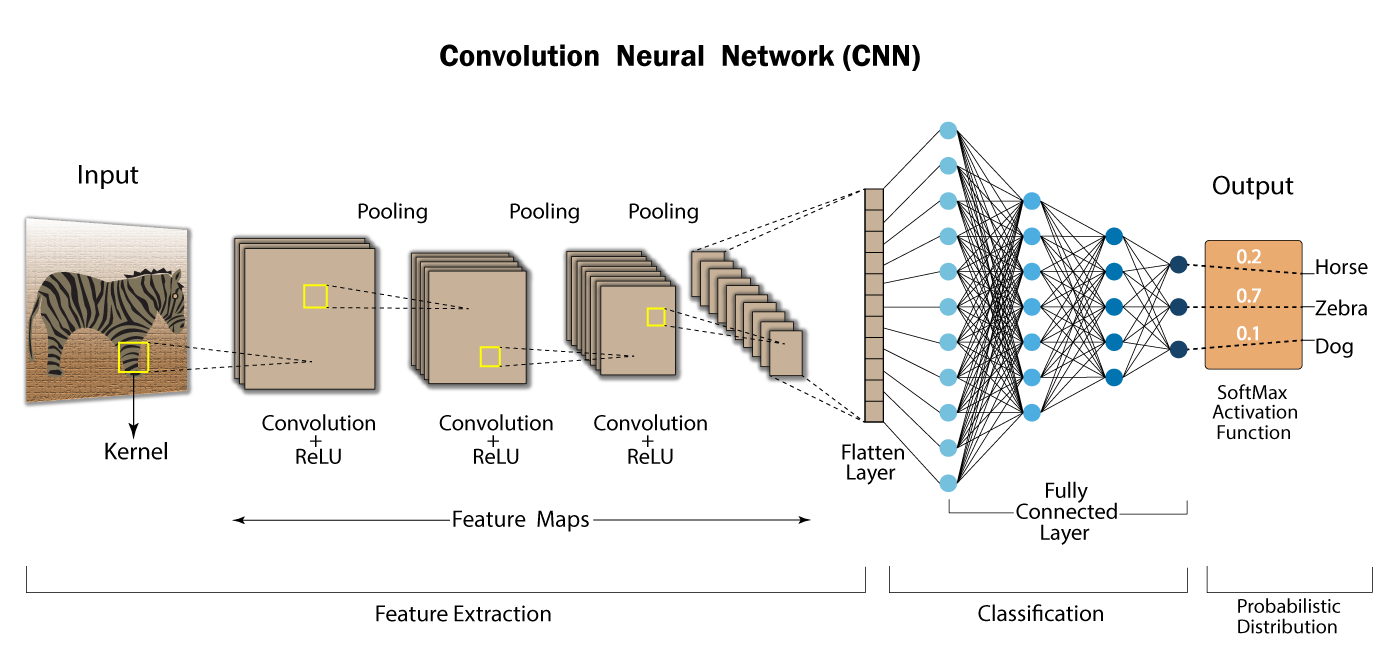
\includegraphics[width=0.85\paperwidth,keepaspectratio]{figures/4_cnn.png}
        
        \vspace{0.5cm}
        \scriptsize\textcolor{gray}{Credit: Swapna @ Developers Breach}
    \end{center}
\end{frame}

%------------------------------------------------
%	NEW SLIDE
%------------------------------------------------
\begin{frame}
    \frametitle{Membedah Gambar: Cara Kerja CNN}
    \framesubtitle{Proses Mengenali Gambar Zebra}
    \small

    \begin{block}{Gambaran Umum}
        Gambar ini memperlihatkan bagaimana \textbf{Convolutional Neural Network (CNN)} mengenali gambar \textbf{Zebra}. Prosesnya terdiri dari dua tahap utama: \textbf{Ekstraksi Fitur} dan \textbf{Klasifikasi}.
    \end{block}

    \begin{itemize}
        \item CNN bekerja seperti "otak digital" yang belajar mengenali objek dalam gambar.
        \item Setiap tahap punya peran khusus, mulai dari mencari ciri-ciri sederhana hingga mengambil keputusan akhir.
    \end{itemize}
\end{frame}

%------------------------------------------------
%	NEW SLIDE
%------------------------------------------------
\begin{frame}
    \frametitle{Tahap 1: Ekstraksi Fitur}
    \framesubtitle{Mencari Ciri-Ciri Penting dalam Gambar}
    \footnotesize

    \begin{center}
        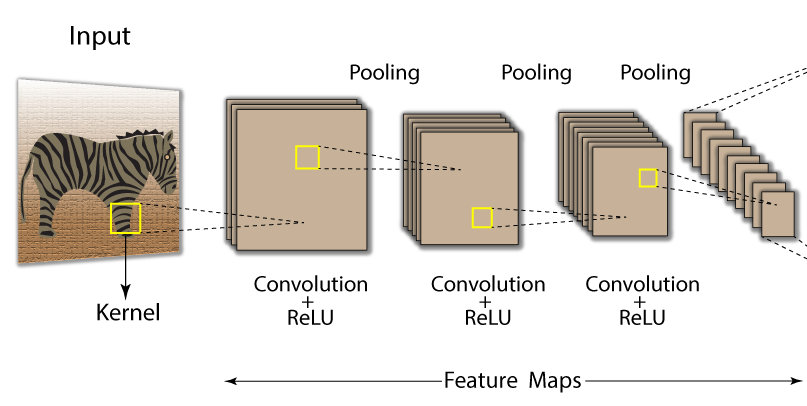
\includegraphics[width=0.45\paperwidth,keepaspectratio]{figures/4_cnn_1.png}
        
        \vspace{0.1cm}
        \scriptsize\textcolor{gray}{Credit: Swapna @ Developers Breach}
    \end{center}

    \begin{block}{Input dan Kernel}
        \textbf{Input} adalah gambar yang ingin dikenali (misal: zebra), yang bagi komputer hanyalah kumpulan angka (piksel). \textbf{Kernel} berfungsi seperti kaca pembesar ajaib yang mencari pola-pola dasar seperti garis atau lengkungan.
    \end{block}

\end{frame}

%------------------------------------------------
%	NEW SLIDE
%------------------------------------------------
\begin{frame}
    \frametitle{Convolution dan Pooling}
    \framesubtitle{Menyaring dan Meringkas Informasi}
    \small

    \begin{block}{Convolution}
        Kernel melakukan \textbf{convolution} dengan menggeser dan memeriksa setiap area gambar, menghasilkan peta ciri untuk setiap pola.
    \end{block}
    
    \begin{itemize}
        \item Kernel bergerak menyisir gambar, mencari pola tertentu.
        \item Hasilnya adalah \textbf{Feature Maps} yang menyorot lokasi pola-pola yang ditemukan.
    \end{itemize}

    \begin{block}{Pooling}
        Pooling bertugas meringkas peta ciri agar hanya informasi penting yang dipertahankan, membuat proses lebih efisien dan robust.
    \end{block}

    \begin{itemize}
        \item Proses convolution dan pooling diulang beberapa kali, sehingga ciri yang dikenali semakin kompleks.
    \end{itemize}
\end{frame}

%------------------------------------------------
%	NEW SLIDE
%------------------------------------------------
\begin{frame}
    \frametitle{Tahap 2: Klasifikasi}
    \framesubtitle{Mengambil Keputusan dari Ciri yang Terkumpul}
    \small

    \begin{center}
        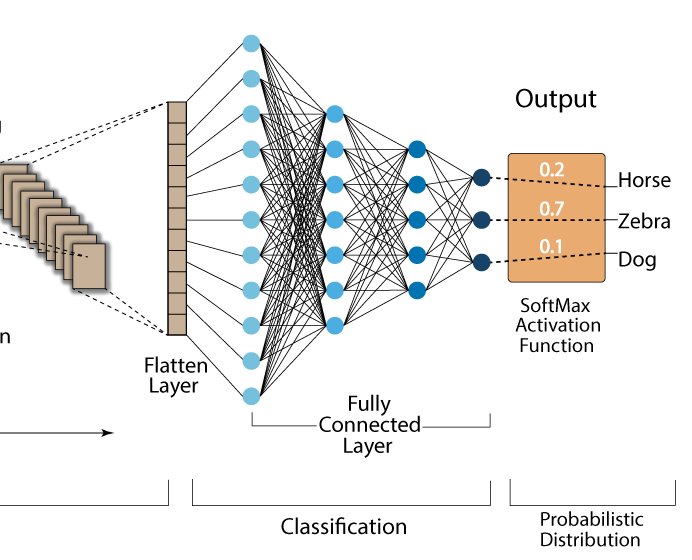
\includegraphics[width=0.25\paperwidth,keepaspectratio]{figures/4_cnn_2.png}
        
        \vspace{0.1cm}
        \scriptsize\textcolor{gray}{Credit: Swapna @ Developers Breach}
    \end{center}

    \begin{block}{Flatten dan Fully Connected Layer}
        Semua peta ciri diratakan menjadi satu baris data panjang (\textbf{flatten}), lalu diproses oleh \textbf{fully connected layer} (otak jaringan) untuk menganalisis dan mengambil keputusan.
    \end{block}


\end{frame}

%------------------------------------------------
%	NEW SLIDE
%------------------------------------------------
\begin{frame}
    \frametitle{Output: Probabilitas Klasifikasi}
    \framesubtitle{Keputusan Akhir CNN}
    \small
    \begin{itemize}
        \item Layer ini menimbang semua ciri yang sudah dikumpulkan.
        \item Proses berpikir: "Ciri-ciri ini cocok dengan objek apa?"
    \end{itemize}
    \begin{block}{Softmax Layer}
        Lapisan terakhir (\textbf{Softmax}) memberikan hasil berupa probabilitas untuk setiap kelas objek.
    \end{block}

    \begin{itemize}
        \item Misal: 70\% yakin gambar adalah Zebra, 20\% Kuda, 10\% Anjing.
        \item Probabilitas tertinggi menjadi jawaban akhir sistem.
    \end{itemize}
\end{frame}

%------------------------------------------------
%	NEW SLIDE
%------------------------------------------------
\begin{frame}
    \frametitle{Kesimpulan Sederhana}
    \framesubtitle{Alur Kerja CNN}
    \small

    \begin{enumerate}
        \item \textbf{Lihat \& Cari Ciri:} Pecah gambar menjadi ciri-ciri dasar (garis, lengkungan).
        \item \textbf{Gabungkan Ciri:} Bentuk ciri kompleks (mata, telinga, pola belang).
        \item \textbf{Simpulkan:} Analisis semua ciri dan tebak objek berdasarkan probabilitas.
    \end{enumerate}

    \begin{block}{Inti CNN}
        CNN belajar mengenali objek dengan mengekstrak ciri-ciri penting dan mengambil keputusan berdasarkan data yang terkumpul.
    \end{block}
\end{frame}

\begin{frame}[plain]
    \begin{center}
        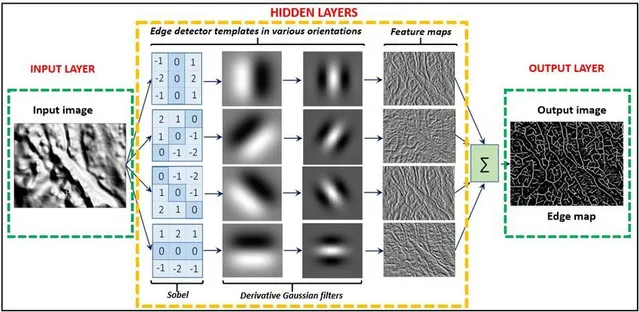
\includegraphics[width=0.85\paperwidth,keepaspectratio]{figures/4_filter.png}
        
        \vspace{0.5cm}
        \scriptsize\textcolor{gray}{Credit: Apurv Chudasama}
    \end{center}
\end{frame}

%------------------------------------------------
%	NEW SLIDE: HIERARCHICAL FEATURE REPRESENTATION
%------------------------------------------------
\begin{frame}
    \frametitle{Representasi Fitur Hierarkis dalam CNN}
    \framesubtitle{Dari Piksel Primitif Menuju Semantik Objek}
    \small

    \begin{block}{Bagaimana CNN Memahami Dunia Visual?}
        Lapisan-lapisan konvolusi yang bertumpuk secara hierarkis mengekstrak representasi visual dari tingkat primitif hingga tingkat semantik tinggi:
    \end{block}

    \begin{columns}[t]
        \column{0.32\textwidth}
        \begin{exampleblock}{\textbf{Layer Awal}}
            \textbf{Low-Level Features}
            \begin{itemize}
                \footnotesize
                \item Tepi (\textit{edges})
                \item Garis vertikal/horizontal
                \item Gradien warna \& kontras
                \item \textit{Biologis: Sel V1 korteks visual mamalia}
            \end{itemize}
        \end{exampleblock}

        \column{0.32\textwidth}
        \begin{block}{\textbf{Layer Tengah}}
            \textbf{Mid-Level Features}
            \begin{itemize}
                \footnotesize
                \item Tekstur (\textit{textures})
                \item Sudut (\textit{corners}) \& kurva
                \item Pola geometris berulang
                \item Motif permukaan objek
            \end{itemize}
        \end{block}

        \column{0.32\textwidth}
        \begin{alertblock}{\textbf{Layer Dalam}}
            \textbf{High-Level Features}
            \begin{itemize}
                \footnotesize
                \item Bagian objek (\textit{parts}): mata, roda, moncong
                \item Struktur semantik utuh
                \item Langsung masuk ke fully connected classifier
            \end{itemize}
        \end{alertblock}
    \end{columns}
\end{frame}

\begin{frame}
    \frametitle{Video Pembelajaran: Operasi Konvolusi dan Pooling}
    \framesubtitle{Tonton di Rumah untuk Pemahaman Mendalam}

    \begin{block}{Tugas Mandiri}
        Silakan tonton video berikut di rumah untuk memperdalam pemahaman tentang operasi konvolusi dan pooling pada CNN:
        \begin{itemize}
            \item \textbf{YouTube:} \href{https://www.youtube.com/watch?v=pj9-rr1wDhM}{Convolution and Pooling Explained}
            \item Link: \href{https://www.youtube.com/watch?v=pj9-rr1wDhM}{https://www.youtube.com/watch?v=pj9-rr1wDhM}
        \end{itemize}
    \end{block}

    \begin{itemize}
        \item Catat poin-poin penting dan contoh yang diberikan dalam video.
        \item Siapkan pertanyaan atau hal yang belum dipahami untuk didiskusikan di kelas berikutnya.
    \end{itemize}
\end{frame}

\section{Perhitungan Matematis di CNN}

\begin{frame}[plain]
  \begin{beamercolorbox}[wd=\paperwidth,ht=\paperheight,sep=1.5cm]{palette primary}
    \vspace{1.5cm}
    {\scriptsize\bfseries\color{dlMute}BAGIAN 04 · MATEMATIKA}\\[0.4cm]
    {\Huge\bfseries Perhitungan Matematis di CNN}\\[0.4cm]
    {\small\color{dlHairline}Memahami Operasi Konvolusi dan Pooling secara Matematis}
    \vfill
  \end{beamercolorbox}
\end{frame}

\begin{frame}
    \frametitle{Perhitungan Matematis CNN}
    \framesubtitle{Dasar-Dasar yang Perlu Dipahami}
    \small

    \begin{block}{Konsep Fundamental}
        CNN tidak "melihat" gambar seperti mata manusia. Bagi komputer, gambar adalah \textbf{matriks angka} dimana setiap angka merepresentasikan intensitas piksel.
    \end{block}

    \begin{columns}[t]
        \column{0.48\textwidth}
        \textbf{Yang Kita Butuhkan:}
        \begin{itemize}
            \item \textbf{Input:} Matriks gambar (misal 5x5)
            \item \textbf{Filter/Kernel:} Matriks kecil (misal 3x3)
            \item \textbf{Operasi:} Konvolusi dan Pooling
        \end{itemize}

        \column{0.48\textwidth}
        \textbf{Tujuan:}
        \begin{itemize}
            \item \textbf{Konvolusi:} Deteksi pola dan fitur
            \item \textbf{Pooling:} Reduksi dimensi
            \item \textbf{Feature Map:} Representasi fitur
        \end{itemize}
    \end{columns}

\end{frame}

%------------------------------------------------
%	NEW SLIDE
%------------------------------------------------
\begin{frame}
    \frametitle{Operasi Konvolusi: Step by Step}
    \framesubtitle{Cara Kerja "Detektif Pola"}
    \footnotesize

    \begin{block}{Input dan Filter}
        Mari kita gunakan contoh sederhana untuk memahami operasi konvolusi.
    \end{block}

    \begin{columns}[t]
        \column{0.48\textwidth}
        \textbf{Input Gambar (5x5):}
        $$
        \begin{pmatrix}
        1 & 1 & 1 & 0 & 0 \\
        0 & 1 & 1 & 1 & 0 \\
        0 & 0 & 1 & 1 & 1 \\
        0 & 0 & 1 & 1 & 0 \\
        0 & 1 & 1 & 0 & 0
        \end{pmatrix}
        $$

        \column{0.48\textwidth}
        \textbf{Filter/Kernel (3x3):}
        $$
        \begin{pmatrix}
        1 & 0 & 0 \\
        0 & 1 & 0 \\
        0 & 0 & 1
        \end{pmatrix}
        $$
        
        \vspace{0.3cm}
        Filter ini mendeteksi pola diagonal (\textbackslash)
    \end{columns}

\end{frame}

%------------------------------------------------
%	NEW SLIDE
%------------------------------------------------
\begin{frame}
    \frametitle{Langkah 1: Element-wise Multiplication}
    \framesubtitle{Perkalian Posisi-Posisi yang Sesuai}
    \footnotesize

    \begin{block}{Posisi Filter di Kiri Atas}
        Letakkan filter di pojok kiri atas input, lalu kalikan elemen yang bersesuaian.
    \end{block}

    $$
    \begin{pmatrix}
    \underline{1 \times 1} & \underline{1 \times 0} & \underline{1 \times 0} & 0 & 0 \\
    \underline{0 \times 0} & \underline{1 \times 1} & \underline{1 \times 0} & 1 & 0 \\
    \underline{0 \times 0} & \underline{0 \times 0} & \underline{1 \times 1} & 1 & 1 \\
    0 & 0 & 1 & 1 & 0 \\
    0 & 1 & 1 & 0 & 0
    \end{pmatrix}
    $$

    \textbf{Hasil perkalian:} $1, 0, 0, 0, 1, 0, 0, 0, 1$

    \textbf{Jumlahkan semua:} $1 + 0 + 0 + 0 + 1 + 0 + 0 + 0 + 1 = 3$

    Angka \textbf{3} ini adalah elemen pertama dari feature map!

\end{frame}

%------------------------------------------------
%	NEW SLIDE
%------------------------------------------------
\begin{frame}
    \frametitle{Langkah 2: Sliding Window (Geser Filter)}
    \framesubtitle{Ulangi untuk Seluruh Area}
    \footnotesize

    \begin{block}{Geser Filter Satu Posisi ke Kanan}
        Ulangi operasi yang sama untuk posisi filter berikutnya.
    \end{block}

    $$
    \begin{pmatrix}
    1 & \underline{1 \times 1} & \underline{1 \times 0} & \underline{0 \times 0} & 0 \\
    0 & \underline{1 \times 0} & \underline{1 \times 1} & \underline{1 \times 0} & 0 \\
    0 & \underline{0 \times 0} & \underline{1 \times 0} & \underline{1 \times 1} & 1 \\
    0 & 0 & 1 & 1 & 0 \\
    0 & 1 & 1 & 0 & 0
    \end{pmatrix}
    $$

    \textbf{Perhitungan:} $(1x1) + (1x0) + (0x0) + (1x0) + (1x1) + (1x0) + (0x0) + (0x1) + (1x1) = 3$

    \begin{itemize}
        \item Lanjutkan proses ini untuk seluruh area gambar
        \item Geser ke kanan, lalu turun satu baris dan ulangi
    \end{itemize}

\end{frame}

%------------------------------------------------
%	NEW SLIDE
%------------------------------------------------
\begin{frame}
    \frametitle{Hasil Konvolusi: Feature Map}
    \framesubtitle{Representasi Fitur yang Terdeteksi}
    \small

    \begin{block}{Feature Map Hasil Konvolusi}
        Setelah filter bergerak ke seluruh area input, kita mendapatkan feature map berukuran 3x3.
    \end{block}

    \begin{center}
        \textbf{Feature Map:}
        $$
        \begin{pmatrix}
        3 & 3 & 1 \\
        1 & 4 & 3 \\
        1 & 3 & 3
        \end{pmatrix}
        $$
    \end{center}

    \textbf{Interpretasi:}
    \begin{itemize}
        \item Nilai besar (seperti \textbf{4}) = pola diagonal sangat kuat terdeteksi
        \item Nilai kecil (seperti \textbf{1}) = pola tidak terlalu cocok
        \item Feature map menunjukkan lokasi dan kekuatan fitur yang dicari
    \end{itemize}

\end{frame}

%------------------------------------------------
%	NEW SLIDE: STRIDE
%------------------------------------------------
\begin{frame}
    \frametitle{Parameter Konvolusi (1): Stride}
    \framesubtitle{Mengontrol Langkah Pergeseran Kernel}
    \small

    \begin{block}{Definisi Stride ($S$)}
        \textbf{Stride} menentukan seberapa jauh (berapa piksel) jendela filter melompat pada setiap pergeseran secara horizontal dan vertikal di atas citra input.
    \end{block}

    \begin{columns}[t]
        \column{0.48\textwidth}
        \textbf{Stride = 1 ($S=1$):}
        \begin{itemize}
            \item Filter bergeser piksel demi piksel (\textit{smooth sliding}).
            \item Ekstraksi fitur sangat padat dan detail.
            \item Ukuran feature map output hanya menyusut sedikit.
            \item Standar pada arsitektur konvolusi klasik.
        \end{itemize}

        \column{0.48\textwidth}
        \textbf{Stride $\ge$ 2 (misal $S=2$):}
        \begin{itemize}
            \item Filter melompati 1 piksel di setiap langkah.
            \item Menghasilkan \textbf{downsampling spasial} (ukuran feature map berkurang sekitar 50\%).
            \item \textbf{Praktik Modern (ResNet/ConvNeXt):} Sering digunakan sebagai pengganti pooling untuk mereduksi dimensi.
        \end{itemize}
    \end{columns}
\end{frame}

%------------------------------------------------
%	NEW SLIDE: PADDING
%------------------------------------------------
\begin{frame}
    \frametitle{Parameter Konvolusi (2): Padding}
    \framesubtitle{Menjaga Dimensi Spasial dan Informasi Tepi}
    \small

    \begin{columns}[t]
        \column{0.48\textwidth}
        \textbf{Mengapa Perlu Padding ($P$)?}
        \begin{itemize}
            \item \textbf{Masalah Penyusutan Spasial:} Tanpa padding, setiap operasi konvolusi akan mengecilkan ukuran citra. Pada network yang dalam, ukuran akan menjadi $1\times1$ terlalu cepat!
            \item \textbf{Masalah Informasi Tepi:} Piksel di sudut hanya disentuh kernel satu kali, sedangkan piksel tengah disentuh berkali-kali.
        \end{itemize}

        \column{0.48\textwidth}
        \textbf{Dua Mode Utama Padding:}
        \begin{itemize}
            \item \textbf{Valid Padding ($P=0$):}
            Tidak ada padding sama sekali. Ukuran output selalu lebih kecil daripada input.
            \item \textbf{Same Padding:}
            Menambahkan border nol (\textit{Zero-Padding}) sedemikian rupa sehingga ukuran output \textbf{sama persis} dengan ukuran input saat $S=1$:
            $$P = \frac{K - 1}{2} \quad (\text{untuk } K \text{ ganjil})$$
            Contoh: Kernel $3\times3 \implies P=1$; Kernel $5\times5 \implies P=2$.
        \end{itemize}
    \end{columns}
\end{frame}

%------------------------------------------------
%	NEW SLIDE: OUTPUT SHAPE FORMULA
%------------------------------------------------
\begin{frame}
    \frametitle{Rumus Matematis Ukuran Feature Map}
    \framesubtitle{Menghitung Dimensi Output Konvolusi 2D}
    \footnotesize

    \begin{columns}[t]
        \column{0.48\textwidth}
        \begin{exampleblock}{Formula Universal Output}
            Input $W_{in}$, kernel $K$, padding $P$, stride $S$:
            $$W_{out} = \left\lfloor \frac{W_{in} - K + 2P}{S} \right\rfloor + 1$$
        \end{exampleblock}
        \begin{itemize}
            \item Berlaku identik untuk tinggi $H_{out}$ dan lebar $W_{out}$.
            \item Simbol $\lfloor \cdot \rfloor$ adalah pembulatan ke bawah (\textit{floor}).
        \end{itemize}

        \column{0.48\textwidth}
        \textbf{Contoh Perhitungan:}
        \begin{itemize}
            \item \textbf{LeNet C1 (Valid):} $W=32, K=5, S=1, P=0$
            $$W_{out} = \lfloor \tfrac{32 - 5 + 0}{1} \rfloor + 1 = \mathbf{28} \implies (28 \times 28)$$
            \item \textbf{Same Conv:} $W=32, K=3, S=1, P=1$
            $$W_{out} = \lfloor \tfrac{32 - 3 + 2}{1} \rfloor + 1 = \mathbf{32} \implies (32 \times 32)$$
            \item \textbf{Stride 2:} $W=32, K=3, S=2, P=1$
            $$W_{out} = \lfloor \tfrac{32 - 3 + 2}{2} \rfloor + 1 = \mathbf{16} \implies (16 \times 16)$$
        \end{itemize}
    \end{columns}
\end{frame}

%------------------------------------------------
%	NEW SLIDE: PARAMETER COUNT FORMULA
%------------------------------------------------
\begin{frame}
    \frametitle{Rumus Jumlah Parameter Layer Konvolusi}
    \framesubtitle{Analisis Matematis Kompleksitas Model pada Volume 3D}
    \footnotesize

    \begin{exampleblock}{Formula Total Parameter Conv2D}
        $$\text{Weights} = K_H \times K_W \times C_{in} \times C_{out}, \qquad \text{Biases} = C_{out}$$
        $$\mathbf{\text{Total Parameter}} = (K_H \times K_W \times C_{in} + 1) \times C_{out}$$
    \end{exampleblock}

    \begin{columns}[t]
        \column{0.48\textwidth}
        \textbf{Contoh Perhitungan Conv2D ($3\times3$):}
        \begin{itemize}
            \item Input RGB ($C_{in} = 3$), $C_{out} = 16$:
            $$\text{Params} = (3 \times 3 \times 3 + 1) \times 16 = \mathbf{448}$$
            \item Input 64 kanal ($C_{in} = 64$), $C_{out} = 128$:
            $$\text{Params} = (3 \times 3 \times 64 + 1) \times 128 = \mathbf{73.856}$$
        \end{itemize}

        \column{0.48\textwidth}
        \begin{alertblock}{Prinsip Penting}
            Ukuran spasial citra ($H \times W$) \textbf{tidak mempengaruhi} jumlah parameter konvolusi! Citra $32\times32$ maupun $1024\times1024$ memakai jumlah parameter yang sama.
        \end{alertblock}
    \end{columns}
\end{frame}

%------------------------------------------------
%	NEW SLIDE: RECEPTIVE FIELD
%------------------------------------------------
\begin{frame}
    \frametitle{Konsep Receptive Field (Medan Reseptif)}
    \framesubtitle{Bagaimana Layer yang Dalam Melihat Konteks Global}
    \footnotesize

    \begin{block}{Definisi Receptive Field (RF)}
        Area spasial pada citra input asli yang berkontribusi terhadap aktivasi suatu neuron pada feature map tertentu.
    \end{block}

    \begin{columns}[t]
        \column{0.48\textwidth}
        \textbf{Pertumbuhan Receptive Field:}
        \begin{itemize}
            \item \textbf{Layer 1 ($3\times3$):} Melihat area $3\times3$ citra asli ($RF=3$).
            \item \textbf{Layer 2 ($3\times3$):} Melihat $3\times3$ dari Layer 1 $\implies \mathbf{5\times5}$ citra asli!
            \item \textbf{Layer 3 ($3\times3$):} Setara melihat $\mathbf{7\times7}$ citra asli.
            \item \textit{Pooling / Stride 2 mempercepat pertumbuhan RF.}
        \end{itemize}

        \column{0.48\textwidth}
        \begin{exampleblock}{Insight CS231n \& VGGNet}
            \textbf{Dua filter $3\times3$ vs satu filter $5\times5$:}
            \begin{itemize}
                \item Keduanya memiliki RF efektif $\mathbf{5\times5}$.
                \item Bobot $1 \times (5\times5) = 25$ parameter.
                \item Bobot $2 \times (3\times3) = \mathbf{18}$ parameter (hemat 28\%!).
                \item Memiliki \textbf{dua non-linearitas (ReLU)}.
            \end{itemize}
        \end{exampleblock}
    \end{columns}
\end{frame}

%------------------------------------------------
%	NEW SLIDE
%------------------------------------------------
\begin{frame}
    \frametitle{Pooling Layer: Konsep Dasar}
    \framesubtitle{Meringkas Informasi Penting}
    \small

    \begin{block}{Tujuan Pooling}
        Pooling berfungsi untuk \textbf{mengurangi ukuran} feature map sambil \textbf{mempertahankan informasi penting}. Ini membuat model lebih efisien dan robust.
    \end{block}

    \begin{columns}[t]
        \column{0.48\textwidth}
        \textbf{Yang Dibutuhkan:}
        \begin{itemize}
            \item Feature map hasil konvolusi
            \item Ukuran window (biasanya 2x2)
            \item Jenis pooling (Max atau Average)
        \end{itemize}

        \column{0.48\textwidth}
        \textbf{Keuntungan:}
        \begin{itemize}
            \item Reduksi parameter
            \item Mengurangi overfitting
            \item Translation invariance
            \item Komputasi lebih cepat
        \end{itemize}
    \end{columns}

\end{frame}

%------------------------------------------------
%	NEW SLIDE
%------------------------------------------------
\begin{frame}
    \frametitle{Max Pooling: "Si Paling Menonjol"}
    \framesubtitle{Ambil Nilai Maksimum dari Setiap Blok}
    \scriptsize

    \begin{block}{Contoh Feature Map (4x4)}
        Mari kita aplikasikan max pooling pada feature map berikut:
    \end{block}

    $$
    \begin{pmatrix}
    3 & 3 & 2 & 1 \\
    1 & 4 & 3 & 0 \\
    1 & 2 & 3 & 3 \\
    0 & 1 & 1 & 0
    \end{pmatrix}
    $$

    \textbf{Bagi menjadi blok 2x2:}
    $$
    \begin{pmatrix}
    \color{blue}3 & \color{blue}3 \\
    \color{blue}1 & \color{blue}4
    \end{pmatrix}
    \begin{pmatrix}
    \color{red}2 & \color{red}1 \\
    \color{red}3 & \color{red}0
    \end{pmatrix}
    $$
    $$
    \begin{pmatrix}
    \color{green}1 & \color{green}2 \\
    \color{green}0 & \color{green}1
    \end{pmatrix}
    \begin{pmatrix}
    \color{orange}3 & \color{orange}3 \\
    \color{orange}1 & \color{orange}0
    \end{pmatrix}
    $$

    \textbf{Max dari setiap blok:} Biru=4, Merah=3, Hijau=2, Oranye=3

\end{frame}

%------------------------------------------------
%	NEW SLIDE
%------------------------------------------------
\begin{frame}
    \frametitle{Average Pooling: "Si Rata-Rata"}
    \framesubtitle{Ambil Nilai Rata-Rata dari Setiap Blok}
    \footnotesize

    \begin{block}{Menggunakan Feature Map yang Sama}
        Kali ini kita hitung rata-rata dari setiap blok 2x2.
    \end{block}

    \textbf{Perhitungan untuk setiap blok:}
    \begin{itemize}
        \item \textcolor{blue}{Blok biru:} $(3+3+1+4) \div 4 = 11 \div 4 = 2.75$
        \item \textcolor{red}{Blok merah:} $(2+1+3+0) \div 4 = 6 \div 4 = 1.5$
        \item \textcolor{green}{Blok hijau:} $(1+2+0+1) \div 4 = 4 \div 4 = 1$
        \item \textcolor{orange}{Blok oranye:} $(3+3+1+0) \div 4 = 7 \div 4 = 1.75$
    \end{itemize}

    \begin{columns}[t]
        \column{0.48\textwidth}
        \textbf{Hasil Max Pooling:}
        $$
        \begin{pmatrix}
        4 & 3 \\
        2 & 3
        \end{pmatrix}
        $$

        \column{0.48\textwidth}
        \textbf{Hasil Average Pooling:}
        $$
        \begin{pmatrix}
        2.75 & 1.5 \\
        1 & 1.75
        \end{pmatrix}
        $$
    \end{columns}

\end{frame}

%------------------------------------------------
%	NEW SLIDE
%------------------------------------------------
\begin{frame}
    \frametitle{Perbandingan Max vs Average Pooling}
    \framesubtitle{Kapan Menggunakan Yang Mana?}
    \small

    \begin{columns}[t]
        \column{0.48\textwidth}
        \textbf{Max Pooling:}
        \begin{itemize}
            \item \textbf{Lebih populer} dalam praktik
            \item Mempertahankan \textbf{fitur terkuat}
            \item Baik untuk deteksi fitur yang \textbf{spars}
            \item Memberikan \textbf{invariance} yang lebih baik
        \end{itemize}

        \textbf{Kapan digunakan:}
        \begin{itemize}
            \item Image classification
            \item Object detection
            \item Ketika fitur yang prominent penting
        \end{itemize}

        \column{0.48\textwidth}
        \textbf{Average Pooling:}
        \begin{itemize}
            \item Mempertahankan informasi \textbf{keseluruhan}
            \item Lebih \textbf{smooth} dalam transisi
            \item Mengurangi \textbf{noise}
            \item Baik untuk texture analysis
        \end{itemize}

        \textbf{Kapan digunakan:}
        \begin{itemize}
            \item Global Average Pooling
            \item Ketika detail halus penting
            \item Saat ingin menghindari overfitting
        \end{itemize}
    \end{columns}

\end{frame}

%------------------------------------------------
%	NEW SLIDE: TRANSLATION INVARIANCE & DIMENSIONALITY REDUCTION
%------------------------------------------------
\begin{frame}
    \frametitle{Mengapa Pooling? Invariansi Translasi \& Reduksi Spasial}
    \framesubtitle{Dua Alasan Krusial Mengapa CNN Sangat Robust}
    \footnotesize

    \begin{columns}[t]
        \column{0.48\textwidth}
        \begin{block}{1. Invariansi Translasi Lokal}
            \textbf{Robust terhadap Pergeseran Objek:}
            \begin{itemize}
                \item Jika objek atau fitur bergeser sedikit (1--2 piksel), aktivasi fitur hanya bergeser di dalam jendela pooling $2\times2$.
                \item Nilai \textbf{maksimum yang diteruskan tetap sama}:
                $$\max(0, 8, 1, 0) = \max(8, 0, 0, 1) = \mathbf{8}$$
                \item CNN fokus pada \textit{"apakah fitur ada"}, bukan posisi presisi sub-pikselnya.
            \end{itemize}
        \end{block}

        \column{0.48\textwidth}
        \begin{exampleblock}{2. Reduksi Dimensi Spasial}
            \textbf{Efisiensi Komputasi \& Memori:}
            \begin{itemize}
                \item Pooling $2\times2$ stride 2 memotong $75\%$ jumlah piksel ($H/2 \times W/2$).
                \item Mengurangi beban memori dan komputasi (FLOPs) secara drastis pada layer berikutnya.
                \item Memperbesar \textbf{effective receptive field} neuron di layer selanjutnya.
            \end{itemize}
        \end{exampleblock}
    \end{columns}
\end{frame}

%------------------------------------------------
%	NEW SLIDE
%------------------------------------------------
\begin{frame}
    \frametitle{Kesimpulan: Alur Matematis CNN}
    \framesubtitle{Dari Input hingga Feature Map}
    \small

    \begin{block}{Ringkasan Proses}
        CNN bekerja melalui serangkaian operasi matematis sederhana yang diulang berkali-kali untuk mengekstrak dan meringkas fitur.
    \end{block}

    \begin{enumerate}
        \item \textbf{Konvolusi:} 
        \begin{itemize}
            \item Sliding window dengan element-wise multiplication
            \item Menghasilkan feature map yang menunjukkan lokasi fitur
        \end{itemize}
        
        \item \textbf{Pooling:}
        \begin{itemize}
            \item Reduksi dimensi dengan max atau average
            \item Mempertahankan informasi penting sambil mengurangi kompleksitas
        \end{itemize}
        
        \item \textbf{Iterasi:}
        \begin{itemize}
            \item Proses ini diulang dengan berbagai filter
            \item Setiap layer mendeteksi fitur yang semakin kompleks
        \end{itemize}
    \end{enumerate}

\end{frame}




\section{Membangun LeNet Architecture di PyTorch}

\begin{frame}[plain]
  \begin{beamercolorbox}[wd=\paperwidth,ht=\paperheight,sep=1.5cm]{palette primary}
    \vspace{1.5cm}
    {\scriptsize\bfseries\color{dlMute}BAGIAN 05 · IMPLEMENTASI}\\[0.4cm]
    {\Huge\bfseries Membangun LeNet Architecture di PyTorch}\\[0.4cm]
    {\small\color{dlHairline}Implementasi CNN dari Awal menggunakan PyTorch}
    \vfill
  \end{beamercolorbox}
\end{frame}

\begin{frame}[plain]
    \begin{center}
        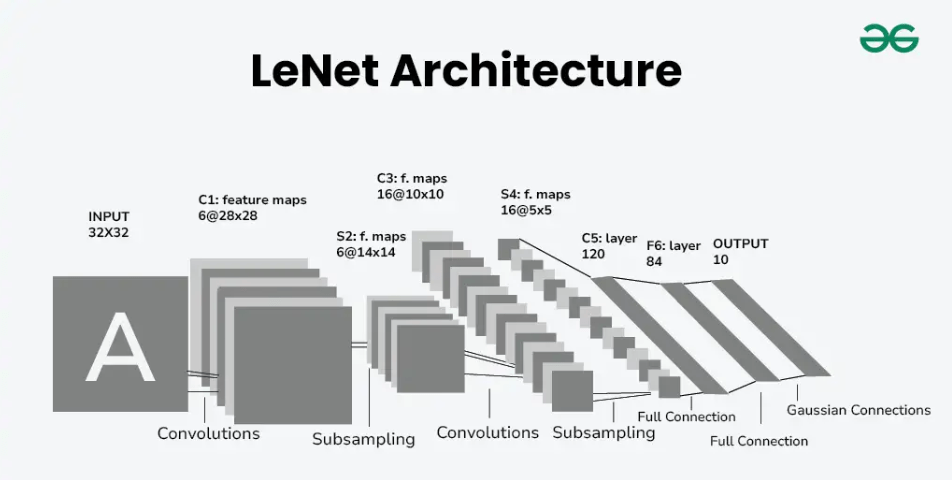
\includegraphics[width=0.85\paperwidth,keepaspectratio]{figures/4_lenet.png}
        
        \vspace{0.5cm}
        \scriptsize\textcolor{gray}{Credit: geeksforgeeks}
    \end{center}
\end{frame}

\begin{frame}
    \frametitle{Yann LeCun: Bapak CNN Modern}
    \framesubtitle{Pelopor Deep Learning dan LeNet}

    \begin{columns}[T]
        \column{0.45\textwidth}
        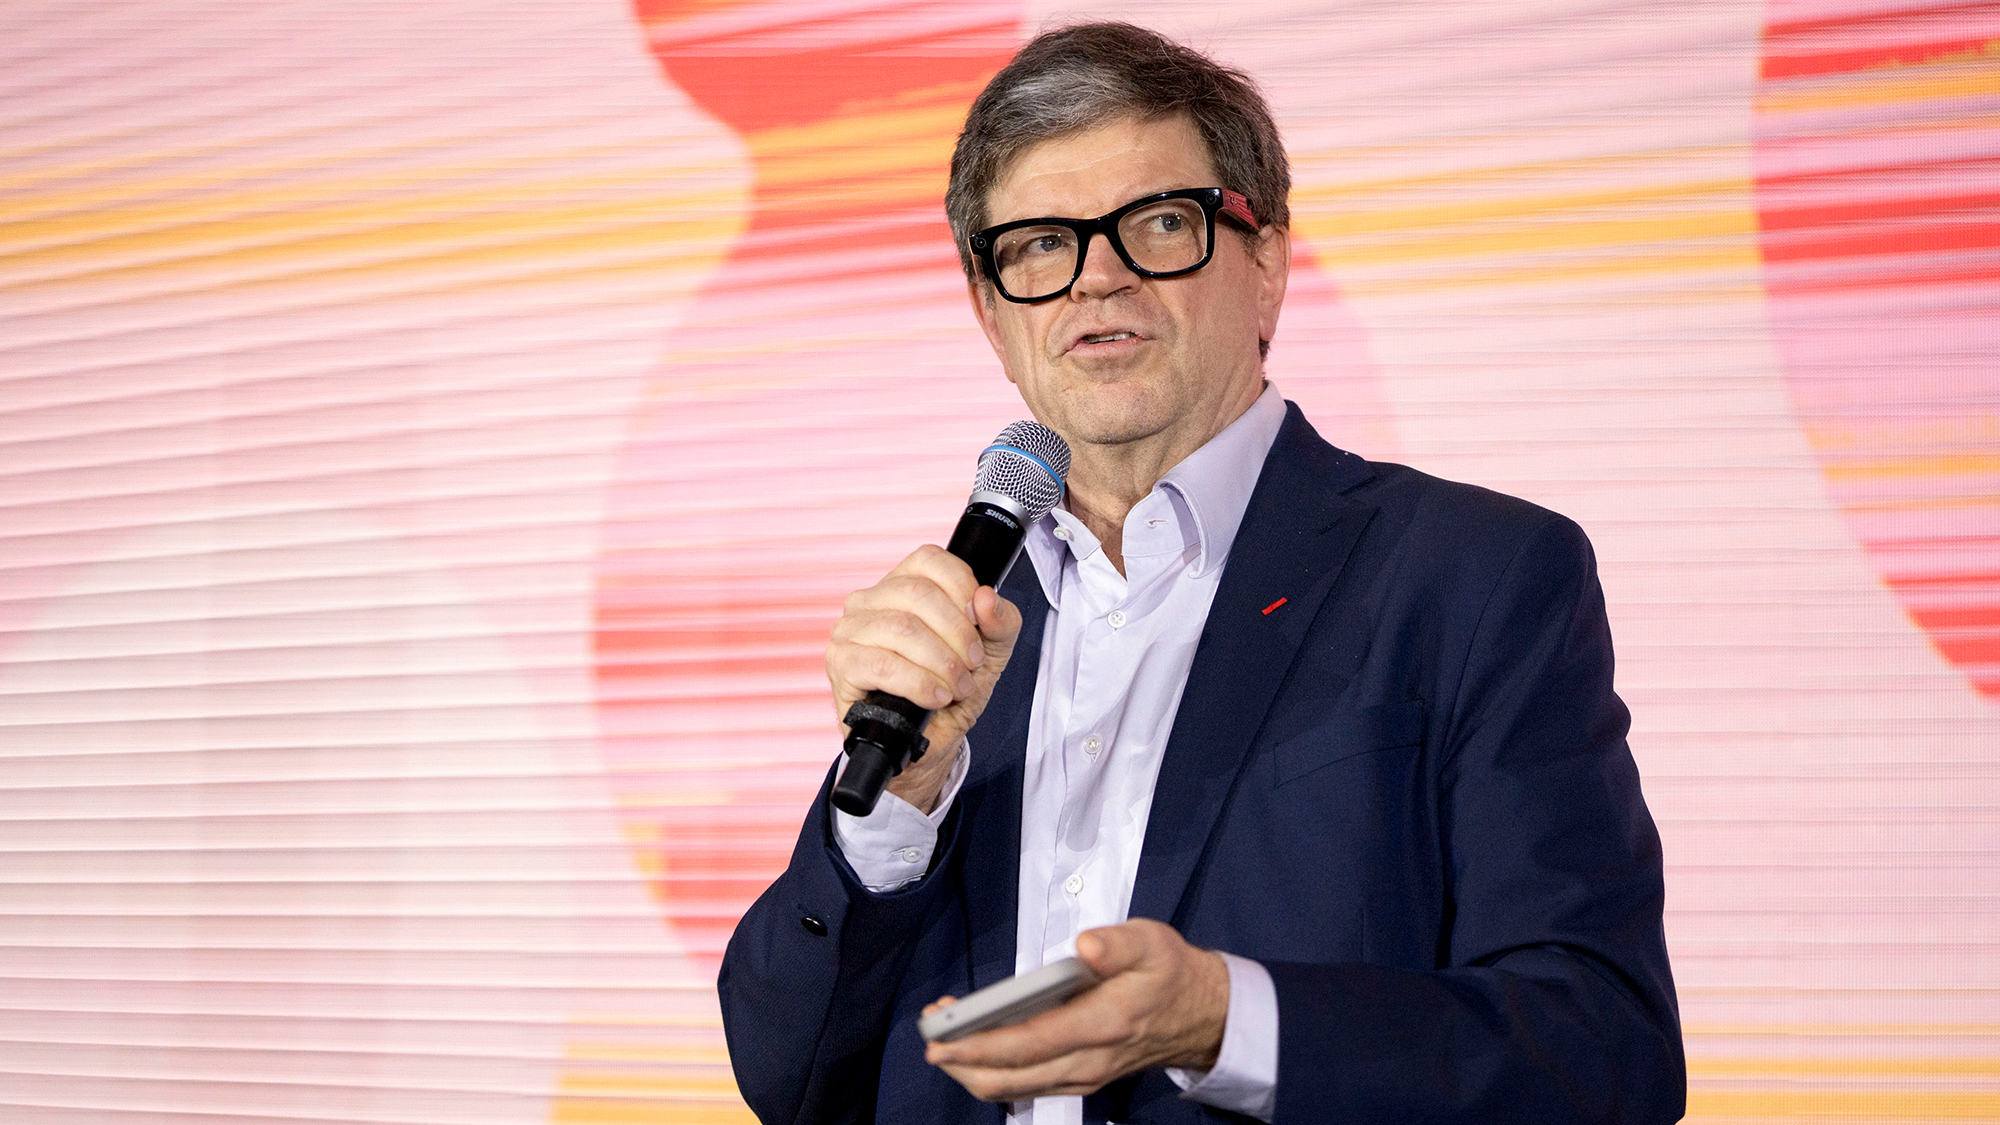
\includegraphics[width=\linewidth]{figures/4_lecun.jpg}
        \vspace{0.2cm}
        \scriptsize\textcolor{gray}{Credit: Bloomberg via Getty Images}

        \column{0.53\textwidth}
        \small
        \textbf{Yann LeCun} adalah ilmuwan komputer asal Prancis yang dikenal sebagai pelopor \textbf{Convolutional Neural Network (CNN)}. Ia menciptakan arsitektur \textbf{LeNet} pada akhir 1980-an, yang menjadi fondasi utama perkembangan deep learning modern, khususnya untuk pengenalan gambar dan tulisan tangan. LeCun juga menerima \textbf{Turing Award 2018} bersama Geoffrey Hinton dan Yoshua Bengio atas kontribusinya di bidang AI.
    \end{columns}
\end{frame}

%------------------------------------------------
%   NEW SLIDE
%------------------------------------------------
\begin{frame}
    \frametitle{Struktur LeNet-5: Overview}
    \framesubtitle{Arsitektur Klasik CNN}
    \small
    \begin{block}{LeNet-5 (Yann LeCun, 1998)}
        LeNet-5 adalah arsitektur CNN klasik yang terdiri dari 7 lapisan utama (tidak termasuk input), dirancang untuk mengenali angka tulisan tangan (MNIST).
    \end{block}
    \begin{itemize}
        \item Input: Gambar 32x32 piksel (MNIST dipadding dari 28x28)
        \item Lapisan: Konvolusi, Pooling, Fully Connected
        \item Output: 10 kelas (digit 0-9)
    \end{itemize}
\end{frame}

%------------------------------------------------
%   NEW SLIDE
%------------------------------------------------
\begin{frame}
    \frametitle{Lapisan C1: Konvolusi Pertama}
    \framesubtitle{Ekstraksi Fitur Dasar}
    \small
    \begin{block}{C1 - Convolutional Layer}
        \begin{itemize}
            \item 6 filter (kernel) berukuran 5x5
            \item Menyapu seluruh gambar input (32x32)
            \item Menghasilkan 6 \textbf{feature maps} berukuran 28x28
            \item Mendeteksi fitur sederhana: tepi, garis, sudut
        \end{itemize}
    \end{block}
\end{frame}

%------------------------------------------------
%   NEW SLIDE
%------------------------------------------------
\begin{frame}
    \frametitle{Lapisan S2: Pooling Pertama}
    \framesubtitle{Subsampling dan Reduksi Dimensi}
    \small
    \begin{block}{S2 - Pooling Layer}
        \begin{itemize}
            \item Pooling (biasanya average pooling) 2x2
            \item Mengurangi ukuran feature map dari 28x28 menjadi 14x14
            \item Jumlah feature map tetap: 6
            \item Membuat model lebih efisien dan robust terhadap pergeseran
        \end{itemize}
    \end{block}
\end{frame}

%------------------------------------------------
%   NEW SLIDE
%------------------------------------------------
\begin{frame}
    \frametitle{Lapisan C3 dan S4: Fitur Kompleks}
    \framesubtitle{Konvolusi Kedua dan Pooling}
    \small
    \begin{columns}[T]
        \column{0.48\textwidth}
        \begin{block}{C3 - Convolutional Layer}
            \begin{itemize}
                \item 16 filter 5x5 pada hasil S2
                \item Output: 16 feature maps berukuran 10x10
                \item Mendeteksi fitur lebih kompleks (kombinasi fitur dasar)
            \end{itemize}
        \end{block}
        \column{0.48\textwidth}
        \begin{block}{S4 - Pooling Layer}
            \begin{itemize}
                \item Pooling 2x2 pada hasil C3
                \item Output: 16 feature maps berukuran 5x5
                \item Reduksi dimensi, tetap 16 maps
            \end{itemize}
        \end{block}
    \end{columns}
\end{frame}

%------------------------------------------------
%   NEW SLIDE
%------------------------------------------------
\begin{frame}
    \frametitle{Lapisan C5 dan F6: Menuju Klasifikasi}
    \framesubtitle{Konvolusi dan Fully Connected}
    \small
    \begin{block}{C5 - Convolutional Layer}
        \begin{itemize}
            \item 120 filter 5x5 pada hasil S4 (input 5x5)
            \item Setiap filter menghasilkan 1 nilai (output 1x1)
            \item Output: 120 neuron (vektor 1D)
        \end{itemize}
    \end{block}
    \begin{block}{F6 - Fully Connected Layer}
        \begin{itemize}
            \item 120 neuron dari C5 terhubung ke 84 neuron
            \item Lapisan ini melakukan proses klasifikasi tingkat tinggi
        \end{itemize}
    \end{block}
\end{frame}

%------------------------------------------------
%   NEW SLIDE
%------------------------------------------------
\begin{frame}
    \frametitle{Lapisan Output: Prediksi Kelas}
    \framesubtitle{Softmax untuk Klasifikasi}
    \small
    \begin{block}{Output Layer}
        \begin{itemize}
            \item 84 neuron F6 terhubung ke 10 neuron output
            \item Setiap neuron mewakili satu kelas (digit 0-9)
            \item Fungsi aktivasi Softmax menghasilkan probabilitas tiap kelas
            \item Prediksi akhir: kelas dengan probabilitas tertinggi
        \end{itemize}
    \end{block}
\end{frame}

%------------------------------------------------
%	NEW SLIDE
%------------------------------------------------
\begin{frame}
    \frametitle{Implementasi LeNet-5 di PyTorch}
    \framesubtitle{Membangun Arsitektur CNN dari Awal}
    \small

    \begin{block}{Tujuan}
        Kita akan mengimplementasikan arsitektur LeNet-5 menggunakan PyTorch dan melihat struktur detail setiap layer dengan \textbf{torchinfo}.
    \end{block}

    \textbf{Yang akan kita pelajari:}
    \begin{itemize}
        \item Definisi kelas LeNet5 dengan PyTorch
        \item Struktur feature extractor dan classifier
        \item Penggunaan torchinfo untuk analisis model
        \item Memahami flow data melalui setiap layer
    \end{itemize}

    \begin{alertblock}{Prasyarat}
        Pastikan sudah menginstall: \texttt{pip install torch torchinfo}
    \end{alertblock}

\end{frame}

%------------------------------------------------
%	NEW SLIDE
%------------------------------------------------
\begin{frame}[fragile]
    \frametitle{Import Libraries dan Setup}
    \framesubtitle{Library yang Diperlukan}
    \small

    \begin{block}{Import Essential Libraries}
\begin{verbatim}
import torch
import torch.nn as nn
from torchinfo import summary
\end{verbatim}
    \end{block}

    \textbf{Penjelasan Library:}
    \begin{itemize}
        \item \texttt{torch}: Core PyTorch library untuk tensor operations
        \item \texttt{torch.nn}: Modul untuk neural network layers dan functions
        \item \texttt{torchinfo}: Library untuk menampilkan summary model yang detail
    \end{itemize}

\end{frame}

%------------------------------------------------
%	NEW SLIDE
%------------------------------------------------
\begin{frame}[fragile]
    \frametitle{Definisi Kelas LeNet5: Constructor}
    \framesubtitle{Inisialisasi Layer-layer CNN}
    \tiny

\begin{verbatim}
class LeNet5(nn.Module):
    """
    Implementasi arsitektur LeNet-5 (1998) menggunakan PyTorch.
    Arsitektur ini didesain untuk input gambar grayscale 32x32 piksel.
    """
    def __init__(self):
        super(LeNet5, self).__init__()

        # === 1. BAGIAN EKSTRAKTOR FITUR ===
        self.feature_extractor = nn.Sequential(
            # Lapisan C1: Konvolusi pertama
            nn.Conv2d(in_channels=1, out_channels=6, kernel_size=5, stride=1),
            nn.Tanh(),
            
            # Lapisan S2: Subsampling (Average Pooling)
            nn.AvgPool2d(kernel_size=2, stride=2),
            
            # Lapisan C3: Konvolusi kedua  
            nn.Conv2d(in_channels=6, out_channels=16, kernel_size=5, stride=1),
            nn.Tanh(),
            
            # Lapisan S4: Subsampling (Average Pooling)
            nn.AvgPool2d(kernel_size=2, stride=2)
        )
\end{verbatim}

\end{frame}

%------------------------------------------------
%	NEW SLIDE
%------------------------------------------------
\begin{frame}[fragile]
    \frametitle{Definisi Kelas LeNet5: Classifier}
    \framesubtitle{Layer Fully Connected untuk Klasifikasi}
    \scriptsize

\begin{verbatim}
        # === 2. BAGIAN KLASIFIKATOR ===
        self.classifier = nn.Sequential(
            # Lapisan C5 (sebagai Fully Connected pertama)
            nn.Linear(in_features=16 * 5 * 5, out_features=120),
            nn.Tanh(),

            # Lapisan F6 (Fully Connected kedua)
            nn.Linear(in_features=120, out_features=84),
            nn.Tanh(),

            # Lapisan Output (10 kelas untuk digit 0-9)
            nn.Linear(in_features=84, out_features=10)
        )
\end{verbatim}

    \textbf{Perhitungan input size untuk Linear layer:}
    \begin{itemize}
        \item Setelah S4: feature maps berukuran 16 x 5 x 5
        \item Flatten: 16 x 5 x 5 = 400 features
        \item Input ke Linear pertama: 400 → 120 → 84 → 10
    \end{itemize}

\end{frame}

%------------------------------------------------
%	NEW SLIDE
%------------------------------------------------
\begin{frame}[fragile]
    \frametitle{Forward Pass Function}
    \framesubtitle{Alur Data Melalui Model}
    \scriptsize

\begin{verbatim}
    def forward(self, x):
        """
        Mendefinisikan alur maju (forward pass) dari data melalui model.
        """
        # Lewatkan input melalui ekstraktor fitur
        x = self.feature_extractor(x)
        
        # Flatten output dari 2D menjadi 1D sebelum masuk ke classifier
        # Dimensi 0 (batch) dipertahankan
        x = torch.flatten(x, 1)
        
        # Lewatkan data yang sudah diratakan melalui classifier
        logits = self.classifier(x)
        return logits
\end{verbatim}

    \textbf{Penjelasan forward pass:}
    \begin{itemize}
        \item Feature extractor: Conv → Pool → Conv → Pool
        \item Flatten: Ubah tensor 4D menjadi 2D untuk FC layers
        \item Classifier: FC → FC → FC (output logits)
    \end{itemize}

\end{frame}

%------------------------------------------------
%	NEW SLIDE
%------------------------------------------------
\begin{frame}[fragile]
    \frametitle{Model Summary dengan Torchinfo}
    \framesubtitle{Analisis Struktur dan Parameter Model}
    \scriptsize

\begin{verbatim}
if __name__ == '__main__':
    # Membuat instance dari model LeNet5
    model = LeNet5()
    
    # Menentukan ukuran input untuk summary
    # Format: (batch_size, channels, height, width)
    input_size = (1, 1, 32, 32) 
    
    # Menampilkan ringkasan model menggunakan torchinfo
    print("=" * 65)
    print("         Ringkasan Arsitektur LeNet-5")
    print("=" * 65)
    summary(model, input_size=input_size)
\end{verbatim}

    \textbf{Input size explanation:}
    \begin{itemize}
        \item Batch size: 1 (untuk testing)
        \item Channels: 1 (grayscale image)
        \item Height x Width: 32 x 32 (sesuai paper LeNet-5)
    \end{itemize}

\end{frame}


%------------------------------------------------
%	NEW SLIDE
%------------------------------------------------
\begin{frame}
    \frametitle{Analisis Output Shape Progression}
    \framesubtitle{Perjalanan Data dari Input ke Output}
    \scriptsize

    \begin{block}{Transformasi Ukuran Data}
        Mari kita trace bagaimana ukuran data berubah melalui setiap layer:
    \end{block}

    \begin{enumerate}
        \item \textbf{Input:} [1, 1, 32, 32] - Batch=1, Channel=1, 32x32 pixels
        \item \textbf{Conv2d C1:} [1, 6, 28, 28] - 6 feature maps, 28x28 each
        \item \textbf{AvgPool S2:} [1, 6, 14, 14] - Ukuran dipotong setengah
        \item \textbf{Conv2d C3:} [1, 16, 10, 10] - 16 feature maps, 10x10 each
        \item \textbf{AvgPool S4:} [1, 16, 5, 5] - Ukuran dipotong setengah lagi
        \item \textbf{Flatten:} [1, 400] - 16x5x5 = 400 features
        \item \textbf{Linear F6:} [1, 120] → [1, 84] → [1, 10]
    \end{enumerate}

    \textbf{Insight:} Dimensi spasial terus mengecil, jumlah channel bertambah.

\end{frame}

%------------------------------------------------
%	NEW SLIDE
%------------------------------------------------
\begin{frame}
    \frametitle{Parameter Count Analysis}
    \framesubtitle{Distribusi Parameter dalam Model}
    \small

    \begin{block}{Total Parameter: 61,706}
        Mari kita breakdown jumlah parameter di setiap layer:
    \end{block}

    \begin{itemize}
        \item \textbf{Conv2d C1:} 156 params = (5x5x1+1)x6 = 26x6
        \item \textbf{Conv2d C3:} 2,416 params = (5x5x6+1)x16 = 151x16
        \item \textbf{Linear C5:} 48,120 params = (400+1)x120 = 401x120
        \item \textbf{Linear F6:} 10,164 params = (120+1)x84 = 121x84
        \item \textbf{Linear Output:} 850 params = (84+1)x10 = 85x10
    \end{itemize}

    \begin{alertblock}{Observasi Penting}
        \textbf{80\%} parameter ada di fully connected layers! Ini menunjukkan mengapa CNN lebih efisien daripada fully connected network biasa.
    \end{alertblock}

\end{frame}

%------------------------------------------------
%	NEW SLIDE
%------------------------------------------------
\begin{frame}
    \frametitle{Keunggulan Implementasi PyTorch}
    \framesubtitle{Fleksibilitas dan Efisiensi}
    \small

    \begin{columns}[t]
        \column{0.48\textwidth}
        \textbf{Keunggulan nn.Sequential:}
        \begin{itemize}
            \item \textbf{Clean code:} Struktur yang rapi
            \item \textbf{Easy debugging:} Layer terorganisir
            \item \textbf{Modular:} Mudah dimodifikasi
            \item \textbf{Automatic forward:} PyTorch handle flow
        \end{itemize}

        \column{0.48\textwidth}
        \textbf{Benefit Torchinfo:}
        \begin{itemize}
            \item \textbf{Visual debugging:} Lihat shape setiap layer
            \item \textbf{Parameter counting:} Hitung kompleksitas
            \item \textbf{Memory analysis:} Estimasi RAM usage
            \item \textbf{Architecture validation:} Cek implementasi
        \end{itemize}
    \end{columns}

    \begin{exampleblock}{Best Practice}
        Selalu gunakan \texttt{torchinfo.summary()} setelah membuat model untuk memverifikasi arsitektur dan mendeteksi potential issues sebelum training.
    \end{exampleblock}

\end{frame}

%------------------------------------------------
%	NEW SLIDE: PYTORCH SETUP TRAINING
%------------------------------------------------
\begin{frame}[fragile]
    \frametitle{Persiapan Pelatihan: Loss \& Optimizer di PyTorch}
    \framesubtitle{Menyiapkan Komponen Pelatihan Model}
    \footnotesize

    \begin{block}{Tiga Komponen Esensial Pelatihan CNN}
        Untuk melatih model CNN dari awal, kita mendefinisikan model, fungsi loss, dan optimizer:
    \end{block}

\begin{verbatim}
model = LeNet5()                                              # Inisialisasi model
criterion = nn.CrossEntropyLoss()                             # Loss multi-kelas
optimizer = torch.optim.Adam(model.parameters(), lr=0.001)    # Optimizer (atau SGD)
\end{verbatim}

    \begin{columns}[t]
        \column{0.48\textwidth}
        \textbf{Fungsi Komponen:}
        \begin{itemize}
            \item \texttt{CrossEntropyLoss}: Gabungan LogSoftmax + NLLLoss untuk klasifikasi.
            \item \texttt{Adam / SGD}: Algoritma pembaruan bobot berbasis gradien.
        \end{itemize}

        \column{0.48\textwidth}
        \textbf{DataLoader:}
        \begin{itemize}
            \item Membagi dataset menjadi \textit{mini-batches} (misal 32 atau 64 citra).
            \item Menyediakan \textit{shuffle} otomatis pada setiap epoch.
        \end{itemize}
    \end{columns}
\end{frame}

%------------------------------------------------
%	NEW SLIDE: PYTORCH TRAINING LOOP
%------------------------------------------------
\begin{frame}[fragile]
    \frametitle{Training Loop CNN di PyTorch}
    \framesubtitle{Alur 5 Langkah Wajib dalam Setiap Batch}
    \scriptsize

\begin{verbatim}
model.train()  # Mode training
for epoch in range(num_epochs):
    for images, labels in train_loader:
        optimizer.zero_grad()               # 1. Reset gradien akumulasi
        outputs = model(images)             # 2. Forward pass: hitung output
        loss = criterion(outputs, labels)   # 3. Hitung loss
        loss.backward()                     # 4. Backward: hitung gradien dL/dw
        optimizer.step()                    # 5. Update bobot (w = w - lr*grad)
\end{verbatim}

    \begin{alertblock}{Penting: Mengapa \texttt{zero\_grad()} Wajib?}
        Secara default di PyTorch, gradien di-\textbf{akumulasi} (\textit{accumulated}). Jika tidak di-reset di awal setiap batch, gradien akan terus bertambah dan merusak arah pembaruan bobot model!
    \end{alertblock}
\end{frame}

%------------------------------------------------
%	NEW SLIDE: PYTORCH EVALUATION
%------------------------------------------------
\begin{frame}[fragile]
    \frametitle{Evaluasi Performa Model (Inference Mode)}
    \framesubtitle{Mengukur Akurasi pada Data Uji (Test Dataset)}
    \scriptsize

\begin{verbatim}
model.eval()  # Mode evaluasi (nonaktifkan behavior training Dropout/BatchNorm)
correct, total = 0, 0

with torch.no_grad():  # Matikan autograd (hemat memori GPU & percepat inferensi)
    for images, labels in test_loader:
        outputs = model(images)
        _, predicted = torch.max(outputs, 1)  # Prediksi kelas probabilitas tertinggi
        total += labels.size(0)
        correct += (predicted == labels).sum().item()

print(f"Akurasi Test Set: {100 * correct / total:.2f}%")
\end{verbatim}

    \begin{exampleblock}{Mengapa \texttt{torch.no\_grad()} Penting Saat Evaluasi?}
        Evaluasi tidak membutuhkan turunan/gradien. \texttt{torch.no\_grad()} mematikan graf komputasi autograd, membebaskan memori RAM/GPU, dan mempercepat inferensi.
    \end{exampleblock}
\end{frame}

%------------------------------------------------
%	NEW SLIDE: SUMMARY OF LEARNING OBJECTIVES
%------------------------------------------------
\begin{frame}
    \frametitle{Ringkasan Pertemuan 4: CNN From Scratch}
    \framesubtitle{Capaian Pembelajaran (RPS IF25-40401)}
    \footnotesize

    \begin{enumerate}
        \item \textbf{Operasi Spasial Citra (Sub-CPMK 1):} Konvolusi mengekstrak representasi spasial; \textbf{Stride ($S$)} langkah geser; \textbf{Padding ($P$)} menjaga border; \textbf{Pooling} mereduksi dimensi \& memberi invariansi translasi.
        \item \textbf{Aritmetika CNN (Sub-CPMK 2):} Output: $O = \lfloor\frac{W - K + 2P}{S}\rfloor + 1$. Parameter: $(K \times K \times C_{in} + 1) \times C_{out}$ (mandiri terhadap resolusi spasial citra input).
        \item \textbf{Pilar Efisiensi vs MLP (Sub-CPMK 4):} \textbf{Local connectivity} + \textbf{Weight sharing} menyelesaikan ledakan jutaan bobot MLP dan menjaga topologi 2D citra.
        \item \textbf{Implementasi PyTorch (Sub-CPMK 3):} LeNet-5 via \texttt{nn.Sequential}, verifikasi bentuk via \texttt{torchinfo}, dan alur 5 langkah training loop.
    \end{enumerate}

    \begin{block}{Persiapan Minggu Depan (Pertemuan 5)}
        \textbf{Deep Computer Vision (2): CNN dan Variasinya} --- Evolusi modern: AlexNet, VGG, ResNet (residual skip connections), MobileNet, dan ConvNeXt.
    \end{block}
\end{frame}

%------------------------------------------------
%	CLOSING SLIDE
%------------------------------------------------
\begin{frame}[plain]
  \begin{beamercolorbox}[wd=\paperwidth,ht=\paperheight,sep=1.5cm]{palette primary}
    \vspace{1.5cm}
    {\scriptsize\bfseries\color{dlMute}IF25-40401 · DEEP LEARNING}\\[0.4cm]
    {\Huge\bfseries Terima Kasih}\\[0.4cm]
    {\small Pertemuan Berikutnya: Deep Computer Vision (2) --- CNN dan Variasinya}\\[1.0cm]
    \vfill
    {\scriptsize\textbf{Tim Dosen Deep Learning} · Institut Teknologi Sumatera (ITERA)}
  \end{beamercolorbox}
\end{frame}

%================================================
%	END DOCUMENT 
%================================================
\end{document}

